\begin{figure}[H]
    \centering\hfill
    \begin{subfigure}{0.4\textwidth}
        \centering
        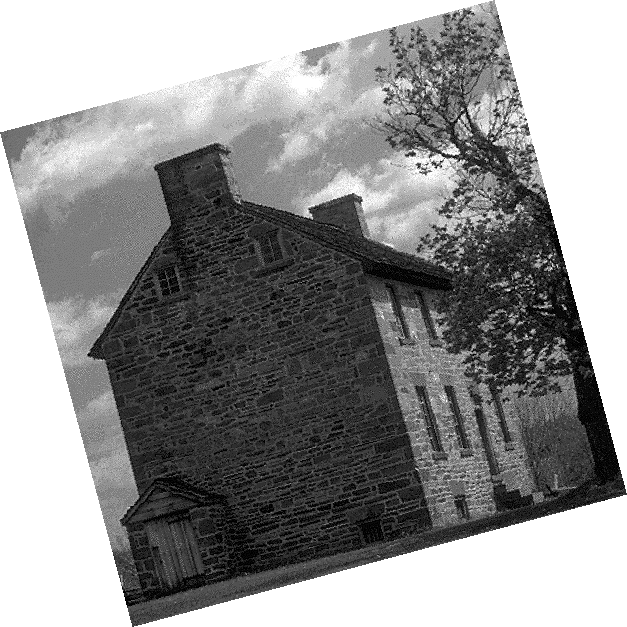
\includegraphics[width=0.9\textwidth]{rotacoes/house_alp_viz.png}
        \caption{~\texttt{vizinho}.}
    \end{subfigure}%
    \hfill%
    \begin{subfigure}{0.4\textwidth}
        \centering
        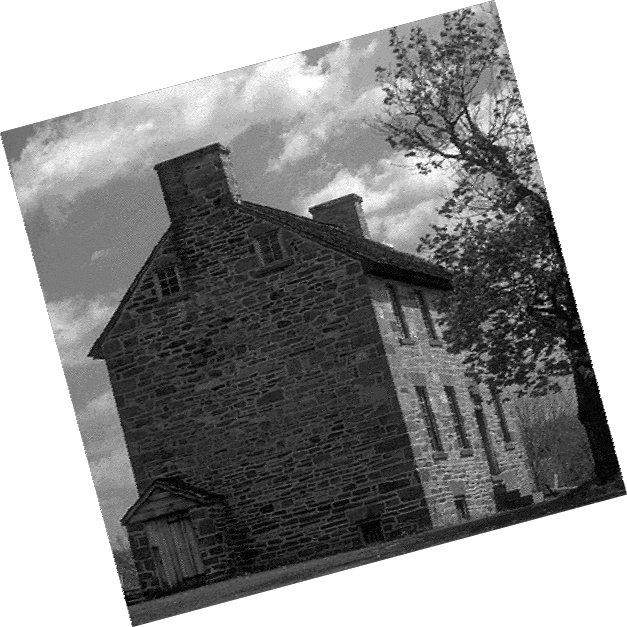
\includegraphics[width=0.9\textwidth]{rotacoes/house_alp_bil.png}
        \caption{~\texttt{bilinear}.}
    \end{subfigure}\hfill
    \\[8pt]\hfill
    \begin{subfigure}{0.4\textwidth}
        \centering
        \includegraphics[width=0.9\textwidth]{rotacoes/house_alp_bic.png}
        \caption{~\texttt{bicubica}.}
    \end{subfigure}%
    \hfill%
    \begin{subfigure}{0.4\textwidth}
        \centering
        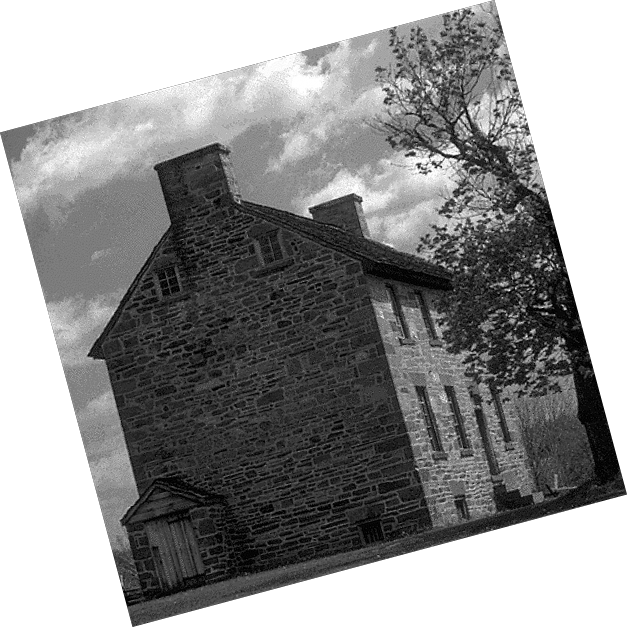
\includegraphics[width=0.9\textwidth]{rotacoes/house_alp_lag.png}
        \caption{~\texttt{lagrange}.}
    \end{subfigure}\hfill

    \caption{Rotação de 15\textdegree{} no plano da imagem aplicada em \texttt{house.png} ($512 \times 512$).}
\end{figure}